

\appendix
\appendixpage
\addappheadtotoc

\section*{A.1) SA-315b Lama main dimensions}
\addcontentsline{toc}{section}{A.1) SA-315b Lama main dimensions}

\bigskip
\begin{figure}[h]
	\begin{center}
		\centering  		 		
		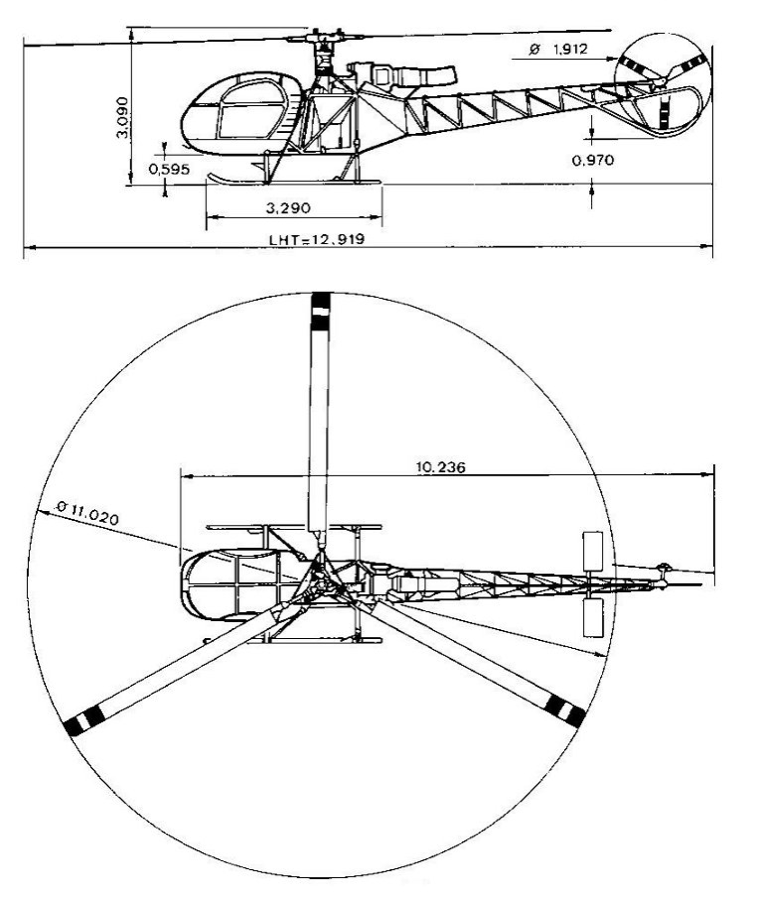
\includegraphics[width=0.90\linewidth]{APPENDIX/PNG/Lama_dimensions.png}
	\end{center}
	\caption {SA-315b Lama main dimensions}
\end{figure}
%\vspace{0.5cm}


\clearpage
\section*{A.2) AS-350 Ecureuil main dimensions}
\addcontentsline{toc}{section}{A.2) AS-350 Ecureuil main dimensions}

\bigskip
\begin{figure}[h]
	\begin{center}
		\centering  		 		
		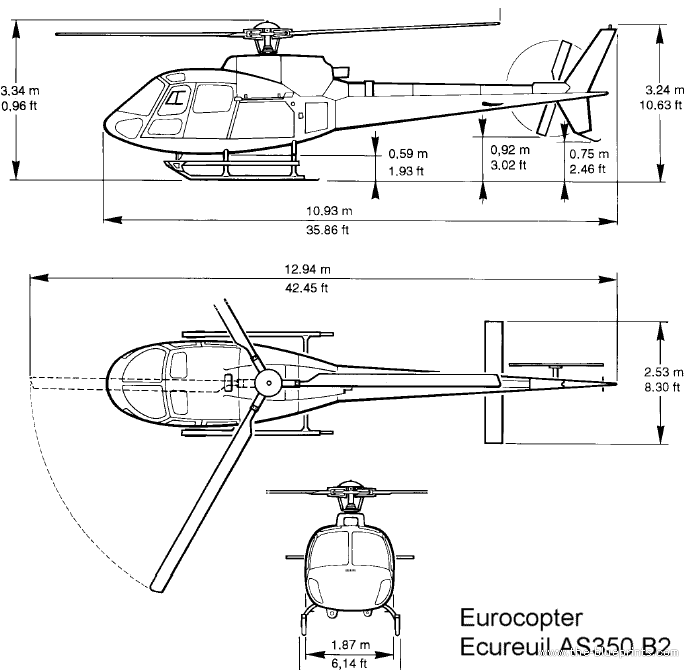
\includegraphics[width=0.90\linewidth]{APPENDIX/PNG/AS-350Ecureuil.png}
	\end{center}
	\caption {AS-350 Ecureuil main dimensions}
\end{figure}
%\vspace{0.5cm}

\clearpage
\section*{A.3) Command lists}
\addcontentsline{toc}{section}{A.3) Command lists}
\bigskip
\subsection*{A.3.1) SA-315b Lama FEM model}
\addcontentsline{toc}{subsection}{A.3.1) SA-315b Lama FEM model (truss)}
\bigskip
\lstinputlisting[language=apdl-modified, caption=2 TAIL MODEL deformazione statica]{./COMMAND_LISTS/2_TAIL_MODEL_deformazione_statica.txt}
\clearpage
\lstinputlisting[language=apdl-modified, caption=4 TAIL MODEL modal analysis tail only CONVERGENCE]{./COMMAND_LISTS/4_TAIL_MODEL_modal_analysis_tail_only_CONVERGENCE.txt}
\lstinputlisting[language=apdl-modified, caption=5 TAIL MODEL GEARBOX SHAFT(lumped approach)]{./COMMAND_LISTS/5_TAIL_MODEL_GEARBOX_SHAFT(lumped_approach).txt}
%
\clearpage
\subsection*{A.3.2) AS-350 Ecureuil FEM model (semi-monocoque)}
\addcontentsline{toc}{subsection}{A.3.2) AS-350 Ecureuil FEM model (semi-monocoque)}
\bigskip
\lstinputlisting[language=apdl-modified, caption=ShellModel]{./COMMAND_LISTS/ShellModel.txt}
\lstinputlisting[language=apdl-modified, caption=ShellModelShaftLumped]{./COMMAND_LISTS/ShellModelShaftLumped.txt}
%
\clearpage
\subsection*{A.3.3) Rotordynamics}
\addcontentsline{toc}{subsection}{A.3.3) Rotordynamics}
\bigskip
\lstinputlisting[language=apdl-modified, caption=RotorTailTransientAnalysis]{./COMMAND_LISTS/RotorTailTransientAnalysis.txt}
\lstinputlisting[language=apdl-modified, caption=6 TAIL MODEL GEARBOX SHAFTRotor]{./COMMAND_LISTS/6_TAIL_MODEL_GEARBOX_SHAFTRotor.txt}
\lstinputlisting[language=apdl-modified, caption=ShellModeldiskStatic]{./COMMAND_LISTS/ShellModeldiskStatic.txt}

%
\clearpage
\subsection*{A.3.4) Macro files}
\addcontentsline{toc}{subsection}{A.3.4) Macro files}
\bigskip
\lstinputlisting[language=apdl-modified, caption=rotorgenrator]{./COMMAND_LISTS/macro/rotor.mac}
\lstinputlisting[language=apdl-modified, caption=skinpersonalization]{./COMMAND_LISTS/macro/testperson.mac}
\lstinputlisting[language=apdl-modified, caption=relativereferencesystem]{./COMMAND_LISTS/macro/relativereferencesystem.mac}
\lstinputlisting[language=apdl-modified, caption=distancenode]{./COMMAND_LISTS/macro/distancenode.mac}
\lstinputlisting[language=apdl-modified, caption=calcmass]{./COMMAND_LISTS/macro/calcmass.mac}
\lstinputlisting[language=apdl-modified, caption=getextremeaxis]{./COMMAND_LISTS/macro/getextremeaxis.mac}